\documentclass[color=usenames,dvipsnames]{beamer}

\mode<presentation> {

\usetheme{Madrid}

\usepackage{tikz}
\usetikzlibrary{shapes.geometric, arrows}

\definecolor{ERC1}{HTML}{C72321}
\definecolor{ERC2}{HTML}{861719}
\definecolor{ERC3}{HTML}{FBD7A9}
\definecolor{ERC4}{HTML}{BA9F7C}
\definecolor{ERC5}{HTML}{7A6952}
\definecolor{ERC6}{HTML}{6E9B9E}
\definecolor{ERC7}{HTML}{0D8085}
\definecolor{ERC8}{HTML}{19484C}
\definecolor{ERC9}{HTML}{F0C320}
\definecolor{ERC10}{HTML}{AF8F19}


\tikzstyle{startstop} = [rectangle, rounded corners, minimum width=3cm, minimum height=1cm,text centered, draw=black, fill=ERC8]
\tikzstyle{io} = [trapezium, text centered, draw=white, fill=white]
\tikzstyle{process} = [rectangle, minimum width=3cm, minimum height=1cm, text centered, draw=black, fill=ERC9]
\tikzstyle{decision} = [diamond, minimum width=3cm, minimum height=1cm, text centered, draw=black, fill=ERC10]
\tikzstyle{arrow} = [thick,->,>=stealth]


\setbeamercolor{palette primary}{bg=ERC1,fg=white}
\setbeamercolor{palette secondary}{bg=ERC2,fg=white}
\setbeamercolor{palette tertiary}{bg=ERC3,fg=white}
\setbeamercolor{palette quaternary}{bg=ERC4,fg=white}
\setbeamercolor{structure}{fg=ERC5} % itemize, enumerate, etc
\setbeamercolor{section in toc}{fg=ERC6} % TOC sections

%gets rid of bottom navigation bars
\setbeamertemplate{footline}[frame number]{}

%gets rid of bottom navigation symbols
\setbeamertemplate{navigation symbols}{}

%gets rid of footer
%will override 'frame number' instruction above
%comment out to revert to previous/default definitions
\setbeamertemplate{footline}{}

% Override palette coloring with secondary
%\setbeamercolor{subsection in head/foot}{bg=UBCgrey,fg=white}


%\usecolortheme{lily}
\useoutertheme{infolines}

}


\usepackage{booktabs} 
\usepackage{tikz}


% Thin fonts
\usepackage{cmbright}
\usepackage[T1]{fontenc}

\definecolor{dark_grey}{gray}{0.5}
%\setbeamercolor{normal text}{fg=dark_grey,bg=white}
\setbeamertemplate{navigation symbols}{}

%\setbeamercolor*{palette primary}{fg=gray!100,bg=gray!10}
%\setbeamercolor*{palette quaternary}{fg=gray!100,bg=gray!10}
%\setbeamercolor*{palette secondary}{fg=gray!100,bg=gray!20}
%\setbeamercolor*{palette tertiary}{fg=gray!100,bg=gray!10}
%\setbeamercolor*{navigation symbols}{fg=white,bg=white}
\usefonttheme{default}


\setbeamertemplate{blocks}[rounded][shadow=false]
%\setbeamercolor{block title}{bg=gray!10}
%\setbeamercolor{block body}{fg=gray,bg=gray!10}
%\setbeamercolor{frametitle}{fg=}

\setbeamertemplate{frametitle}[default][center]

\setbeamertemplate{itemize items}[default]
\setbeamertemplate{enumerate items}[default]

\newcommand{\F}{\mathbb{F}}

\setbeamertemplate{title page}[default][colsep=-4bp,rounded=true]

\title[Workshop - Machine Learning]{ Don't believe the hype? A hands-on introduction to machine-learning in Python}
\subtitle{Open Workshops on Computer Based Systems Modelling}

\author{Johannes Schmidt, Johann Baumgartner}
\institute{Institute for Sustainable Economic Development, BOKU, Vienna}
\date{7.05.2019}
\begin{document}

{
\usebackgroundtemplate{
 \begin{picture}(320,315)
 \hspace{6.9cm}
   \includegraphics[width=0.7\linewidth]{../figures/refuel_logo_with_text.png}
 \end{picture}
 }


\begin{frame}

\maketitle



\end{frame}
}
% Uncomment these lines for an automatically generated outline.
%\begin{frame}{Outline}
%  \tableofcontents
%\end{frame}

\section{Contents}

\begin{frame}{Contents - Workshop}

\begin{itemize}
  \item Day 1: Introduction to Machine Learning
  \item Day 2: Understanding backpropagation and Neural Networks in Python
  \item Day 3: An example of a practical application of Neural Networks for image recognition in Python and Reinforcement learning in Python
  \item Day 4: Bring your own data!
\end{itemize}

\end{frame}


\begin{frame}{Contents - Today} 

\begin{itemize}
	\item The basic concept of machine learning
	\item Some examples of machine learning
	\item Supervised, unsupervised, reinforcement learning: practical exercises
	
	\item An introduction to neural networks 

	\begin{itemize}
		\item Basic concepts and terminology
		\item Backpropagation algorithm and its computational complexity
		\item Regression and Classification with neural networks vs. linear models
		\item Under- and overfitting of neural networks
		\item Practical aspects of machine learning
	\end{itemize}

\end{itemize}

%\vskip 1cm

%\begin{block}{Examples}
%Some examples of commonly used commands and features are included, to help you get started.
%\end{block}



\end{frame}

\section{The basic concept of machine learning}


\begin{frame}{The basic concept of machine learning} 


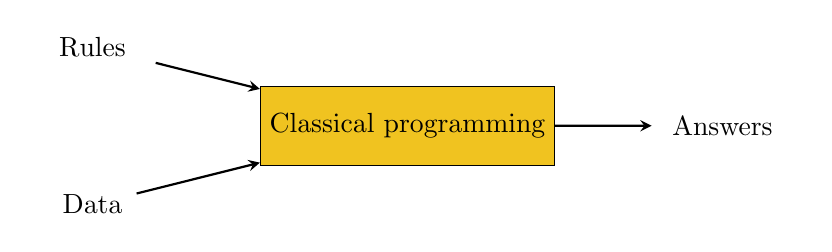
\begin{tikzpicture}[node distance=2cm]

%\node (Start) [startstop] {Start};

\node (in1) [io] {Rules};
\node (in2) [io, below of=in1] {Data};


\node (pro1) [process, right of=in1, xshift = 2cm, yshift = -1cm] {Classical programming};

\node (out1) [io, right of=pro1, xshift = 2cm] {Answers};

\draw [arrow] (in1) -- (pro1);
\draw [arrow] (in2) -- (pro1);

\draw [arrow] (pro1) -- (out1);


\end{tikzpicture}

\vspace{1cm}

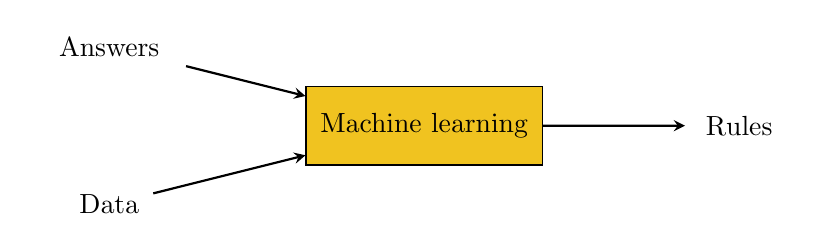
\begin{tikzpicture}[node distance=2cm]

%\node (Start) [startstop] {Start};

\node (in1) [io] {Answers};
\node (in2) [io, below of=in1] {Data};


\node (pro1) [process, right of=in1, xshift = 2cm, yshift = -1cm] {Machine learning};

\node (out1) [io, right of=pro1, xshift = 2cm] {Rules};

\draw [arrow] (in1) -- (pro1);
\draw [arrow] (in2) -- (pro1);

\draw [arrow] (pro1) -- (out1);


\end{tikzpicture}



%\vskip 1cm

%\begin{block}{Examples}
%Some examples of commonly used commands and features are included, to help you get started.
%\end{block}

\end{frame}

\begin{frame}{Why is this cool?} 


\begin{itemize}
	
	\item \href{https://www.captionbot.ai/}{\underline{Image recognition with captionbot.ai}}\\
			(deep learning)\\

	\item \href{https://www.youtube.com/watch?time_continue=2&v=TmPfTpjtdgg}{\underline{Computer plays atari computer games}}\\ 
			(deep learning for 	pattern recognition, deep reinforcement learning)\\

	\item \href{https://youtu.be/rOL6QJdAlm8?t=103}{\underline{The moment alphaGo wins against Lee Sedol}}\\
			(supervised learning and deep reinforcement learning)\\
			
	\item \href{https://www.thispersondoesnotexist.com/}This person does not exist\\
		(Generative adversial network)
	
	\item \href{https://www.predpol.com/}{Predicting where crime occurs}\\
		(Regression model)\\
		
	\item Supervising Oktoberfest waiters
	
\end{itemize}

\end{frame}

\section{Terminology}


\begin{frame}{A typology of machine learning} 


\begin{itemize}
	
	\item Supervised learning: Given inputs and outputs, find the rules that link the two
	\item Unsupervised learning: Find structure in data
	\item Reinforcement learning: learning by doing.
	
\end{itemize}

\end{frame}

\begin{frame}{Supervised learning - Exercise (I)} 



\begin{table}[ht]
	\centering
	\begin{tabular}{c|c}
		Positives&Negatives\\
		\includegraphics[width=0.1\linewidth]{../figures/1d_pattern_supervised_learning_1.png}
		\includegraphics[width=0.1\linewidth]{../figures/1d_pattern_supervised_learning_2.png}
		\includegraphics[width=0.1\linewidth]{../figures/1d_pattern_supervised_learning_3.png}
		\includegraphics[width=0.1\linewidth]{../figures/1d_pattern_supervised_learning_4.png}&
		\includegraphics[width=0.1\linewidth]{../figures/1d_random_supervised_learning_1.png}
		\includegraphics[width=0.1\linewidth]{../figures/1d_random_supervised_learning_2.png}
		\includegraphics[width=0.1\linewidth]{../figures/1d_random_supervised_learning_3.png}
		\includegraphics[width=0.1\linewidth]{../figures/1d_random_supervised_learning_4.png}
		\\
	\end{tabular}
\end{table}

\begin{center}
Positive or Negative?\\
\includegraphics[width=0.1\linewidth]{../figures/1d_pattern_supervised_learning_5.png}
\end{center}

\end{frame}


\begin{frame}{Supervised learning needs labeled datasets} 

\begin{itemize}
	\item Classification. Input features: Photos of people. Labels: smiling or not.
	\item Classification. Photos of waiters carrying plates and glasses. Output: number of plates and glasses.
    \item Classification. Input: German text. Output: English text.
	\item Regression. Input: wind speeds. Output: measured wind power generation.
	\item Therefore: 
		\href{https://www.theverge.com/2019/3/28/18285572/prison-labor-finland-artificial-intelligence-data-tagging-vainu}{\underline{Inmates in Finland are training AI as part of prison labor}}
\end{itemize}

\end{frame}


\begin{frame}{Unsupervised learning - Exercise} 

\begin{center}
	Which data points belong to each other?\\
\includegraphics[width=0.8\linewidth]{../figures/clustering.png}
\end{center}


\end{frame}

\begin{frame}{Unsupervised learning - Find structure in data} 

\begin{itemize}
	\item Clustering (which data belongs together?)
	\item Anomaly detection (which data is somehow strange?)
	\item Generative adversial networks (Generate photos, sounds, and text, also involves supervised learning)
\end{itemize}

\end{frame}


\begin{frame}{Reinforcement learning - Exercise} 

See Netlogo

\end{frame}






{
\usebackgroundtemplate{
 \begin{picture}(320,315)
 \hspace{6.9cm}
   \includegraphics[width=0.7\linewidth]{../figures/refuel_logo_with_text.png}
 \end{picture}
 }


\begin{frame}
\frametitle{Thank you!}
\begin{block}{
 For updates on the project, check \textbf{refuel.world}\\
 For source-code, check \textbf{github.com/joph/MachineLearningCourse}\\
 
		mail: johannes.schmidt@boku.ac.at\\

}
\end{block}

\vspace{2.5 cm}


\end{frame}

}


\end{document} 